\documentclass[tikz, border=10pt]{standalone}
\usepackage{tikz}
\usetikzlibrary{shapes.multipart, arrows.meta}
\usepackage{color}
\tikzset{
state/.style={
       rectangle split,
       rectangle split parts=4,
       rectangle split part fill={violet!30,blue!20,green!20,black!20},
       rectangle split part align={center, center, center, center},
%       rounded corners,
       draw=black,%, very thick,
%       minimum height=2em,
       text width=3cm,
      inner sep=.33cm,
       text centered,
       }
}
\begin{document}

     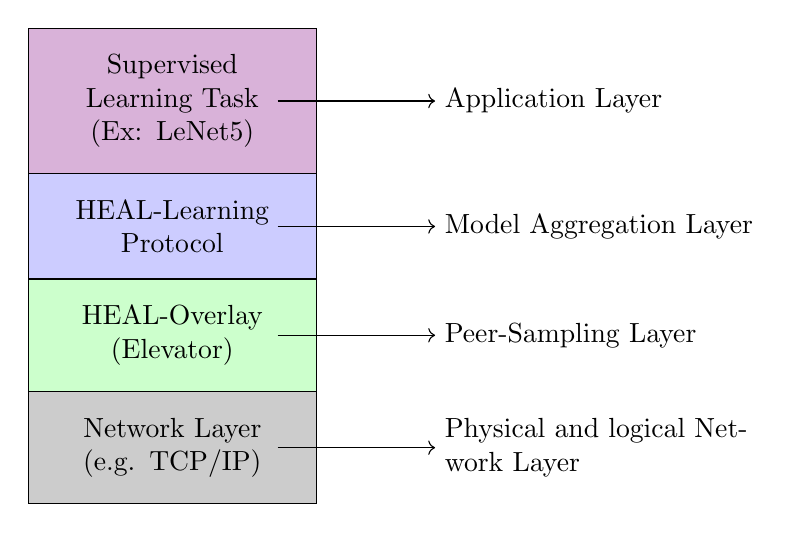
\begin{tikzpicture}
      \node [state] (box) at (0,0) {
                Supervised Learning Task (Ex: LeNet5)
                \nodepart{two}
                HEAL-Learning Protocol
                \nodepart{three}
                HEAL-Overlay (Elevator)
                \nodepart{four}
                Network Layer (e.g. TCP/IP)
            };
    
            % Draw arrows with labels
            \foreach \n/\l in {
                text/Application Layer, 
                two/Model Aggregation Layer, 
                three/Peer-Sampling Layer,
                four/Physical and logical Network Layer
            } {
                \draw[->] ([xshift=-0.5cm]box.\n\space east) -- ++(2,0) node[right, text width=4cm] {\l};
            }
    \end{tikzpicture}
\end{document}
